\documentclass[tikz]{standalone}
\usepackage{tikz}
\usepackage{pgfplots}
\pgfplotsset{compat=1.17}
\begin{document}
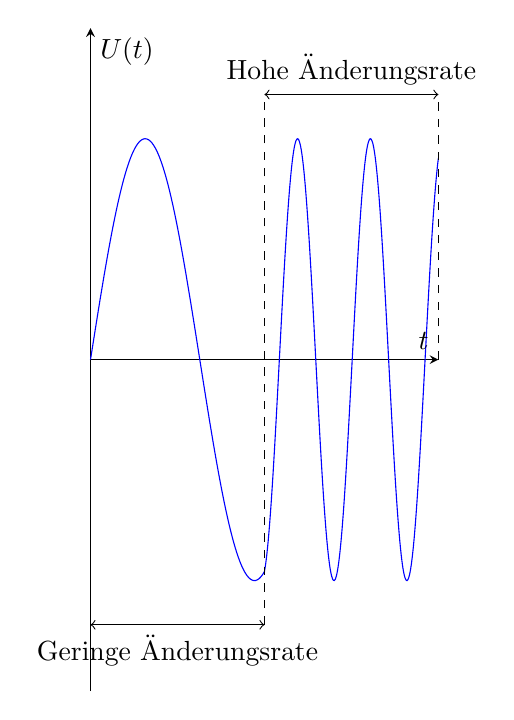
\begin{tikzpicture}
    \begin{axis}[
        width=6cm, height=10cm,
        axis lines=middle,
        xlabel=$t$,
        ylabel={$U(t)$},
        xtick=\empty,
        ytick=\empty,
        xmin=0, xmax=10,
        ymin=-1.5, ymax=1.5,
        clip=false,
    ]
        \addplot[domain=0:5, samples=100, smooth, blue] {sin(deg(x))};
        \addplot[domain=5:10, samples=200, smooth, blue] {sin(deg(3*(x-5)+5))};

        % Markierungen für Phasen
        \draw [dashed] (5,-1.2) -- (5, 1.2);
        \draw [dashed] (10,0) -- (10, 1.2);
        \draw [<->] (0,-1.2) -- (5,-1.2) node [midway,below] {Geringe Änderungsrate};
        \draw [<->] (5,1.2) -- (10,1.2) node [midway,above] {Hohe Änderungsrate};
    \end{axis}
\end{tikzpicture}
\end{document}
